\documentclass{article}
\usepackage{amsfonts}
\usepackage{amsthm}
\usepackage{amssymb}
\usepackage{amsmath}
\usepackage{graphicx}
\usepackage{subcaption}
\usepackage{xcolor}
\usepackage{mathtools}
\usepackage{ wasysym }
\usepackage{enumerate}
\usepackage{verbatim}
\usepackage{hyperref}


\newcommand{\new}[2]{
    \vspace{2mm}
    \noindent
    \textbf{
    \underline{#1}}
    \textit{{#2}}
    \
}

\def\<{{\langle}}
\def\>{{\rangle}}

\DeclarePairedDelimiter\bra{\langle}{\rvert}
\DeclarePairedDelimiter\ket{\lvert}{\rangle}
\DeclarePairedDelimiterX\braket[2]{\langle}{\rangle}{#1\,\delimsize\vert\,\mathopen{}#2}


\newcommand{\textOr}{
    {
        \hspace{5mm}
        \textrm{or}
        \hspace{5mm}
    }
}

\newcommand{\textAnd}{
    {
        \hspace{5mm}
        \textrm{and}
        \hspace{5mm}
    }
}


\newcommand{\textWhere}{
    {
        \hspace{5mm}
        \textrm{where}
        \hspace{5mm}
    }
}



\newcommand{\Ixp}[1]{
    {
        e^{i{#1}}
    }
}



\newcommand{\halfFigure}[1]{
\begin{center}
\includegraphics[width = .5\linewidth]{{#1}}
\end{center}
}

\newcommand{\fullFigure}[1]{
\begin{center}
\includegraphics[width = .9\linewidth]{{#1}}
\end{center}
}

\def\twobytwoMat(#1, #2, #3, #4){
    {
        \begin{bmatrix}
            {#1} & {#2}\\
            {#3} & {#4}
        \end{bmatrix}
    }
}

\def\twobyoneMat(#1, #2){
    {
        \begin{bmatrix}
            {#1}\\
            {#2}
        \end{bmatrix}
    }
}

\def\twobytwoDet(#1, #2, #3, #4){
    {
        \begin{vmatrix}
            {#1} & {#2}\\
            {#3} & {#4}
        \end{vmatrix}
    }
}


\newcommand{\RR}{\mathbb{R}}
\newcommand{\CC}{\mathbb{C}}
\newcommand{\ZZ}{\mathbb{Z}}
\newcommand{\Zpos}{\mathbb{Z}_{pos}}
\newcommand{\NN}{\mathbb{N}}

\newtheorem{theorem}{Theorem}
\newtheorem{proposition}{Proposition}
\newtheorem{lemma}{Lemma}
\newtheorem{corollary}{Corollary}
\newtheorem{remark}{Remark}
\newtheorem{definition}{Definition}
\newtheorem{example}{Example}
\newtheorem{conjecture}{Conjecture}
\newtheorem{question}{Question}

\newcommand{\ch}{\text{ch}}

\begin{document}
\begin{center}
    \Large
    \textbf{Topology Pset 1}

    \large
    Daniel Son
\end{center}

\section{Problem 1: Hex game}
\begin{question}
Rigorously define a Hex game, and prove that the game always have a winner. 
\end{question}

\begin{proof}[Solution]
    A Hex game starts with an empty board comprised of Hexagons. The hexagons are arranged in a shape resembling a parallelogram as described in the figure \ref{fig:HexBoard}. 
    \begin{figure}[h]
        \centering
        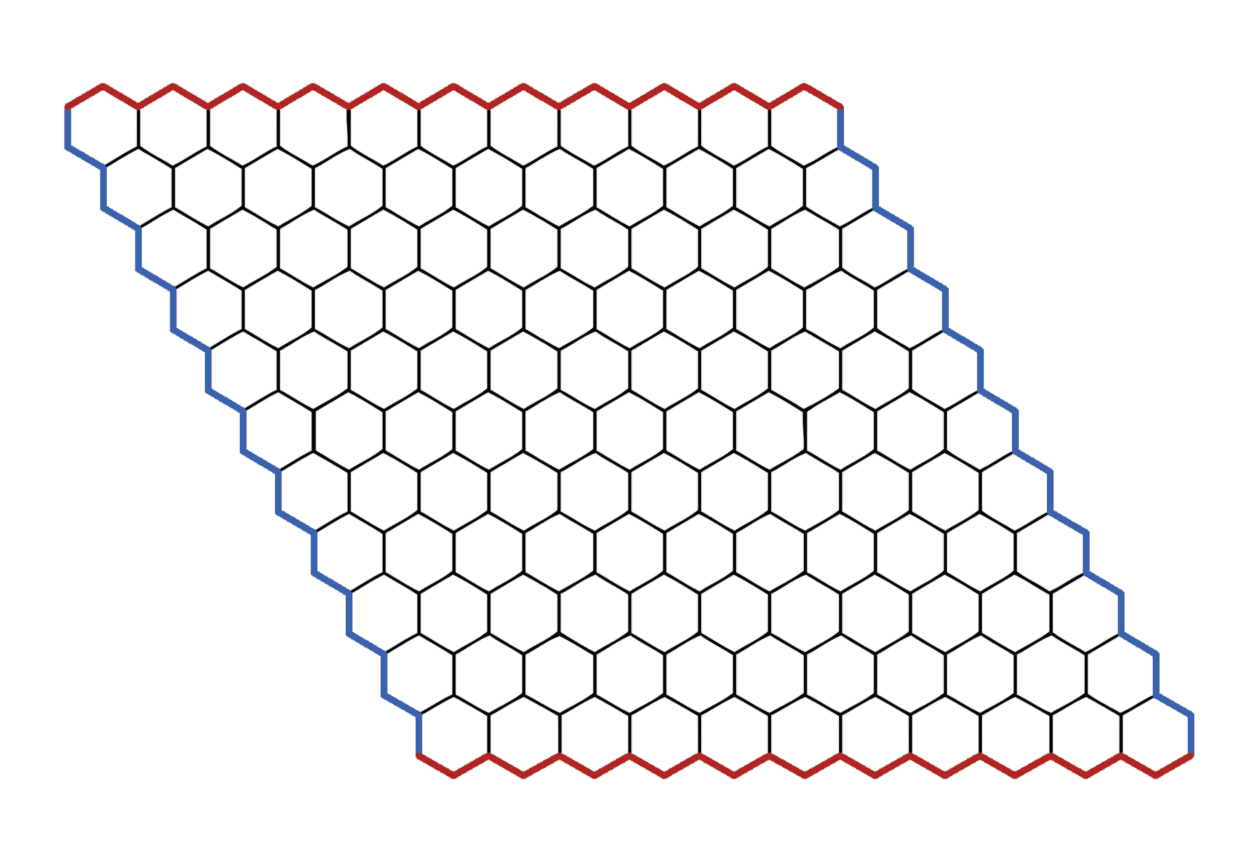
\includegraphics[width=0.8\textwidth]{HexBoard.png} % Replace 'figure.jpg' with your image file
        \caption{An empty Hex board}
        \label{fig:HexBoard}
    \end{figure}
    
    The top and the bottom sides of the parallelogram are assumed to be covered in red, and the right and the left sides in blue. Note that contrary to the figure, we assign the color to the outer region of the board, not the edges. On each turn, a player can take any blank hexagon, and color it either blue or red. The goal of each player is to connect either the top-bottom red reigoins or the right-left blue regions with a path of continuous hexagons. 

    We are asked to prove that a hex game always terminates with a winner. We observe that it suffices to show, for any coloring of the board in red and blue, there exists a chain of hexagons of same color that connects either the top-bottom or the right-left regions. 

    We provide a rigorous definiton of a fully colored board. 

\begin{definition}[Colored Hex Board]
    A colored Hex board is a collection of colored Hexagons arranged in the form of %Figure. 
    Each hexagon either has a color of blue or red. We call each vertex of the hexagons as \textbf{junctions}. A junction where three hexagons meet are called \textbf{regular junctions} . A junction where two hexagons meet are called \textbf{edge junctions}. Finally, a junction that is adjacent to one hexagon is called a \textbf{vertex junction}. 
\end{definition}

We intend to draw out a line that demarks the boundary between the two colors. We precisely define what a boundary edge is. 

\begin{definition}[Boundary edge] Any edge of a hexagon in a colored hex board is a \textbf{boundary edge} if either the edge is adjacent to both a blue hexagon and a red hexago, blue hexagon and a red region outside the board, red hexagon and a blue region outside the board.  
\end{definition}

Through brute forcing all possible cases, we can deduce how many boundary edges are connected to each junction. 
\begin{proposition}\label{thm:bdrycdn}
    Each vertex junction has exactly one adjacent boundary edge. For regular junctions and edge junctions, there exist exactly zero or two adjacent boundary edges. 
\end{proposition}
\begin{proof}
    All cases are listed out in Figure \ref{fig:junctionCases}. Without loss of generality, we can fix the color of the outer regions for the vertex and edge junctions. 
    The boundary edges are marked by green. 
\end{proof}

\begin{figure}[htp]
    \centering
    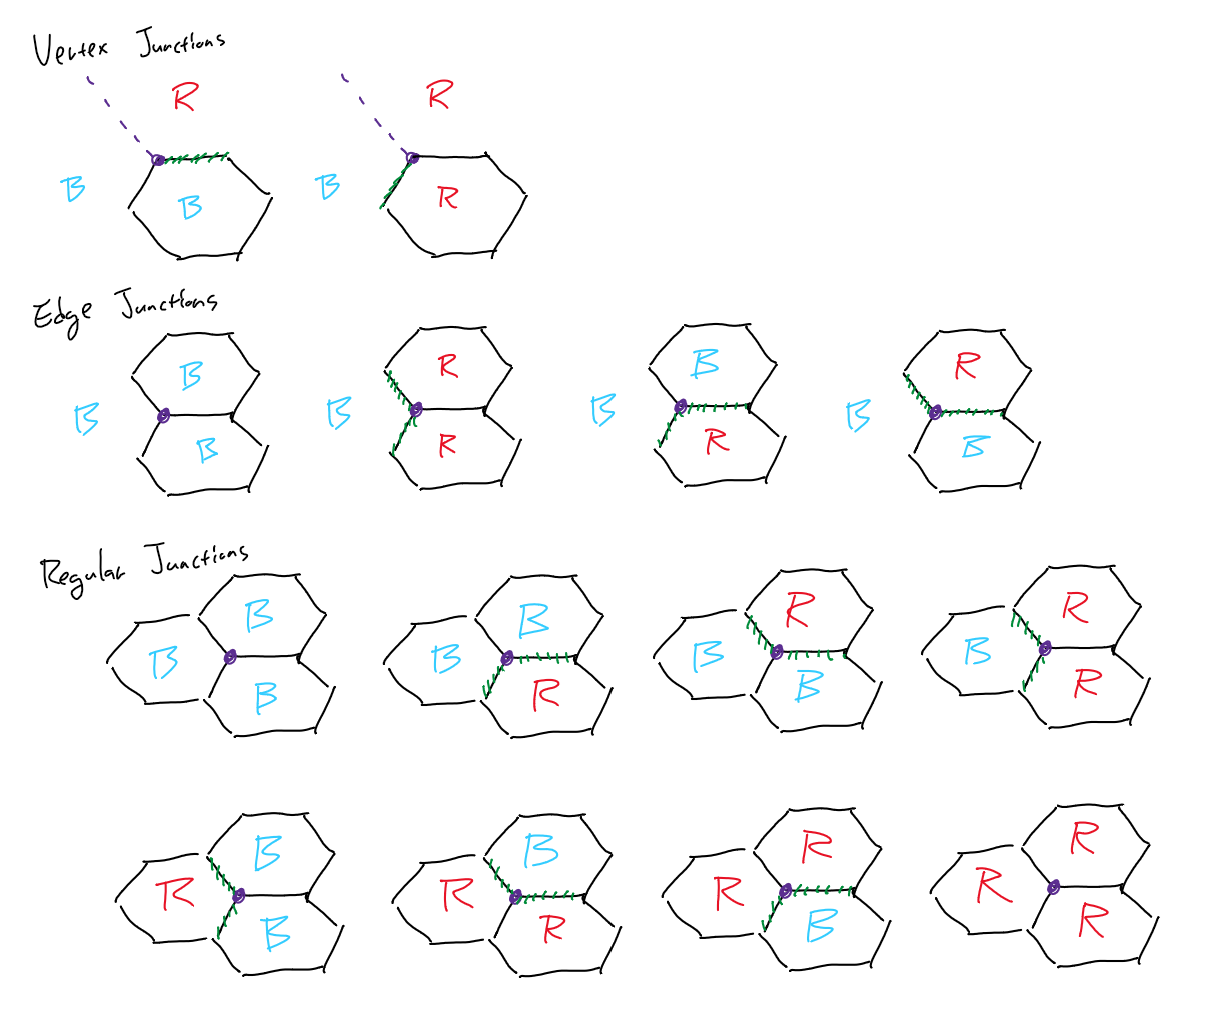
\includegraphics[width=0.8\textwidth]{JunctionCases.png} % Replace 'figure.jpg' with your image file
    \caption{All possible colorings of junctions}
    \label{fig:junctionCases}
\end{figure}

We construct a boundary chain by the following method. 
\begin{definition}[Boundary chains]
    Let $a_0$ be the top-left vertex junction. By Proposition \ref{thm:bdrycdn}, for each junction $a_i$ we obtain a unique $a_{i+1}$ such that the edge connecting these two consecutive junction is a boundary edge. The next junction can be obtained unless $a_n$ for $n > 0$ is a vertex junction, which in case the sequence terminates. A boundary chain is the sequence of junctions $\{a_i\}_{0 \leq i \leq n}$ where $a_0, a_n$ are distinct vertex junctions. 
\end{definition} 

We link our observation on boundaries to chains of hexagons
\begin{proposition}
    If a boundary chain connects two outer regions, there exists a sequence of hexagons, both blue and red, that connect two outer regions. 
\end{proposition}

\begin{proof}
    From the boundary chain $\{a_i\}_{0\leq i \leq n}$, choose the longest continuous subsequence of junctions that are regular junctions and call the subsequence $\{a_i\}_{s \leq i \leq e}$ where $s > 0$ and $e < n$. $a_{s - 1}$ and $a_{e + 1}$ are assumed to be adjacent with some outer region, and thus there exist a chain of boundary edges that connects the two regions. 

    It remains to show that these two regions are of same color and that there exists a consecutive set of same-colored hexagons adjacent to the edges. Without loss of generality, suppose the boundary edges connect a red outer region to a blue outer region. The first boundary edge must connect vertically down from the northern red region. All the hexagons to the right side of the chain must be red. When the last boundary edge connects to the blue region on the right, we reach a contradiction, for the left top red hexagon generates a boundary edge with the blue region, resulting in an edge junction with three adjacent boundary edges. 
    
    The latter claim can be proved by contradiction. From the edge path, one side must be occupoied with red hexagons and the other with blue. Otherwise, if there exists a side where there are both red and blue hexagons directly adjacent to the path, the boundary chain will change, leading to a contradiction. 
\end{proof}

We have proved the following. 

\begin{theorem}
    A game of Hex must terminate, where either player 1 or player 2 successfully connects the two red or blue outer regions with a sequence of consecutively adjacent hexagons with same colors. 
\end{theorem}

\end{proof}

\section{Problem 2: Colinear lines}

\begin{question}[Perspective triangles]
    Fix a point $O$ in $\mathbb R^2$. Two points $A, A'$ in the plane 
    are perspective if they lie on the same line through $O$. 
    Consider three pairs of colinear lines $(A, A')$, $(B, B')$, and $(C, C')$. 
    Construct three points $X, Y, Z$ according to the following definition. 

    \[
X := \overrightarrow{AB} \cap \overrightarrow{A'B'} \quad, \quad
Y := \overrightarrow{AC} \cap \overrightarrow{A'C'} \quad, \quad
Z := \overrightarrow{BC} \cap \overrightarrow{B'C'}
\]
prove that $X, Y, Z$ are colinear. 

\end{question}
\begin{proof}
    Consider the two triangles to resemble a plane in $R^3$. Under 
    the assumption that none of the three pair of lines used to 
    construct $X, Y, Z$ are not parallel to each other, the two planes 
    corresponding to each triangles must not be parallel. 
    $X, Y, Z$ clearly lives on both planes, and two distinct nonparallel 
    planes must meet in one line. $X, Y, Z$ all lives in this one line, 
    and hence they are colinear. 
\end{proof}

\section{Problem 3: playing with paper}
\begin{proof}[Report]
    For part a), c), I constructed a diagram that characterized 
    the paper strip. I conjectured that cutting the strip in half 
    will yield in one paper strip with \textbf{0-twist} and 
    cutting the strip in thirds will yield two paper strips both with 
    a \textbf{1-twist}. The crux of my argument is that the rotation of 
    the paper preserves its topological properties. 
    \begin{figure}[h]
        \centering
        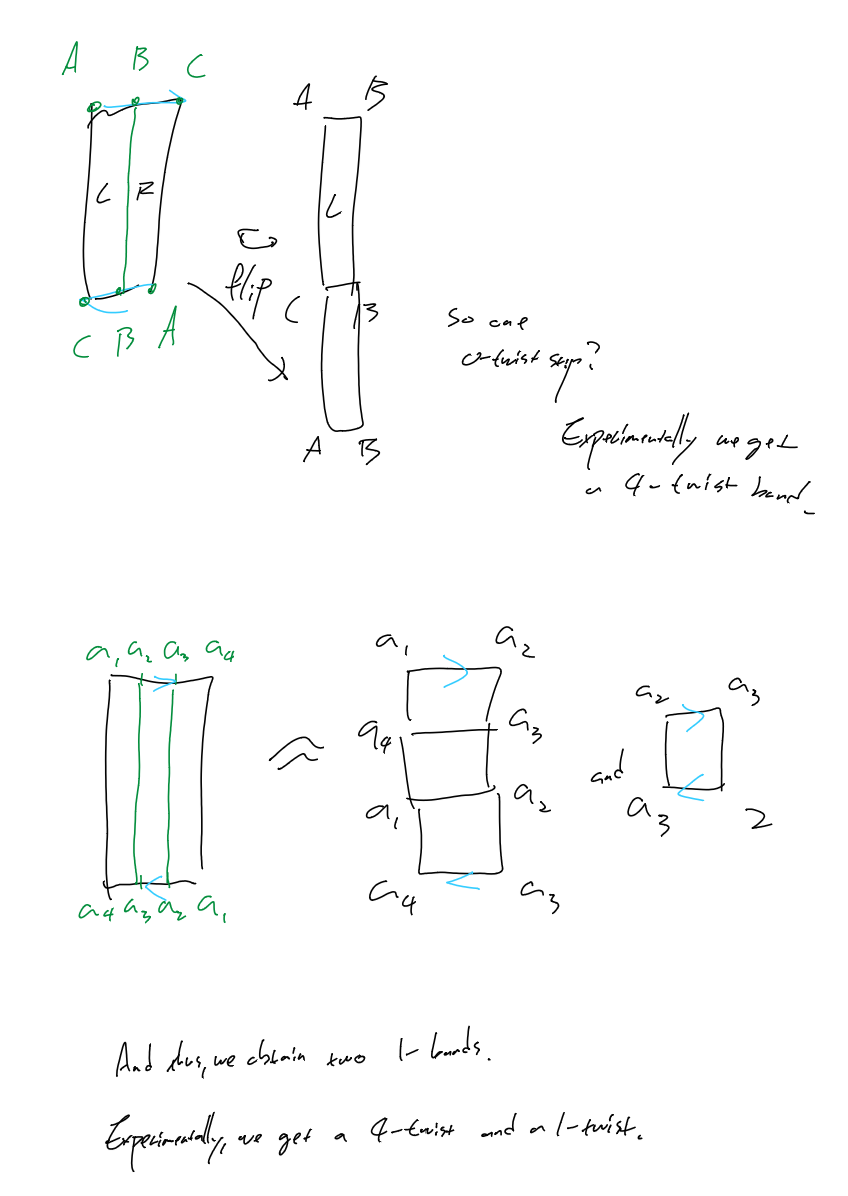
\includegraphics[width=0.8\textwidth]{conjectures.png} % Replace 'figure.jpg' with your image file
        \caption{Diagrams for my conjecture}
        \label{fig:conjectures}
    \end{figure}
    For experimental verification, I slices a strip of A4 paper 
    and stabled them together. Before ripping through each 
    piece of paper, I marked the anticipated path with a pen. 
    After the cut, I tore one section of the strip, and continued rotating to 
    measure the type of the strip. 

    \begin{figure}[htp]
        \centering
        \begin{subfigure}[b]{0.45\textwidth}
            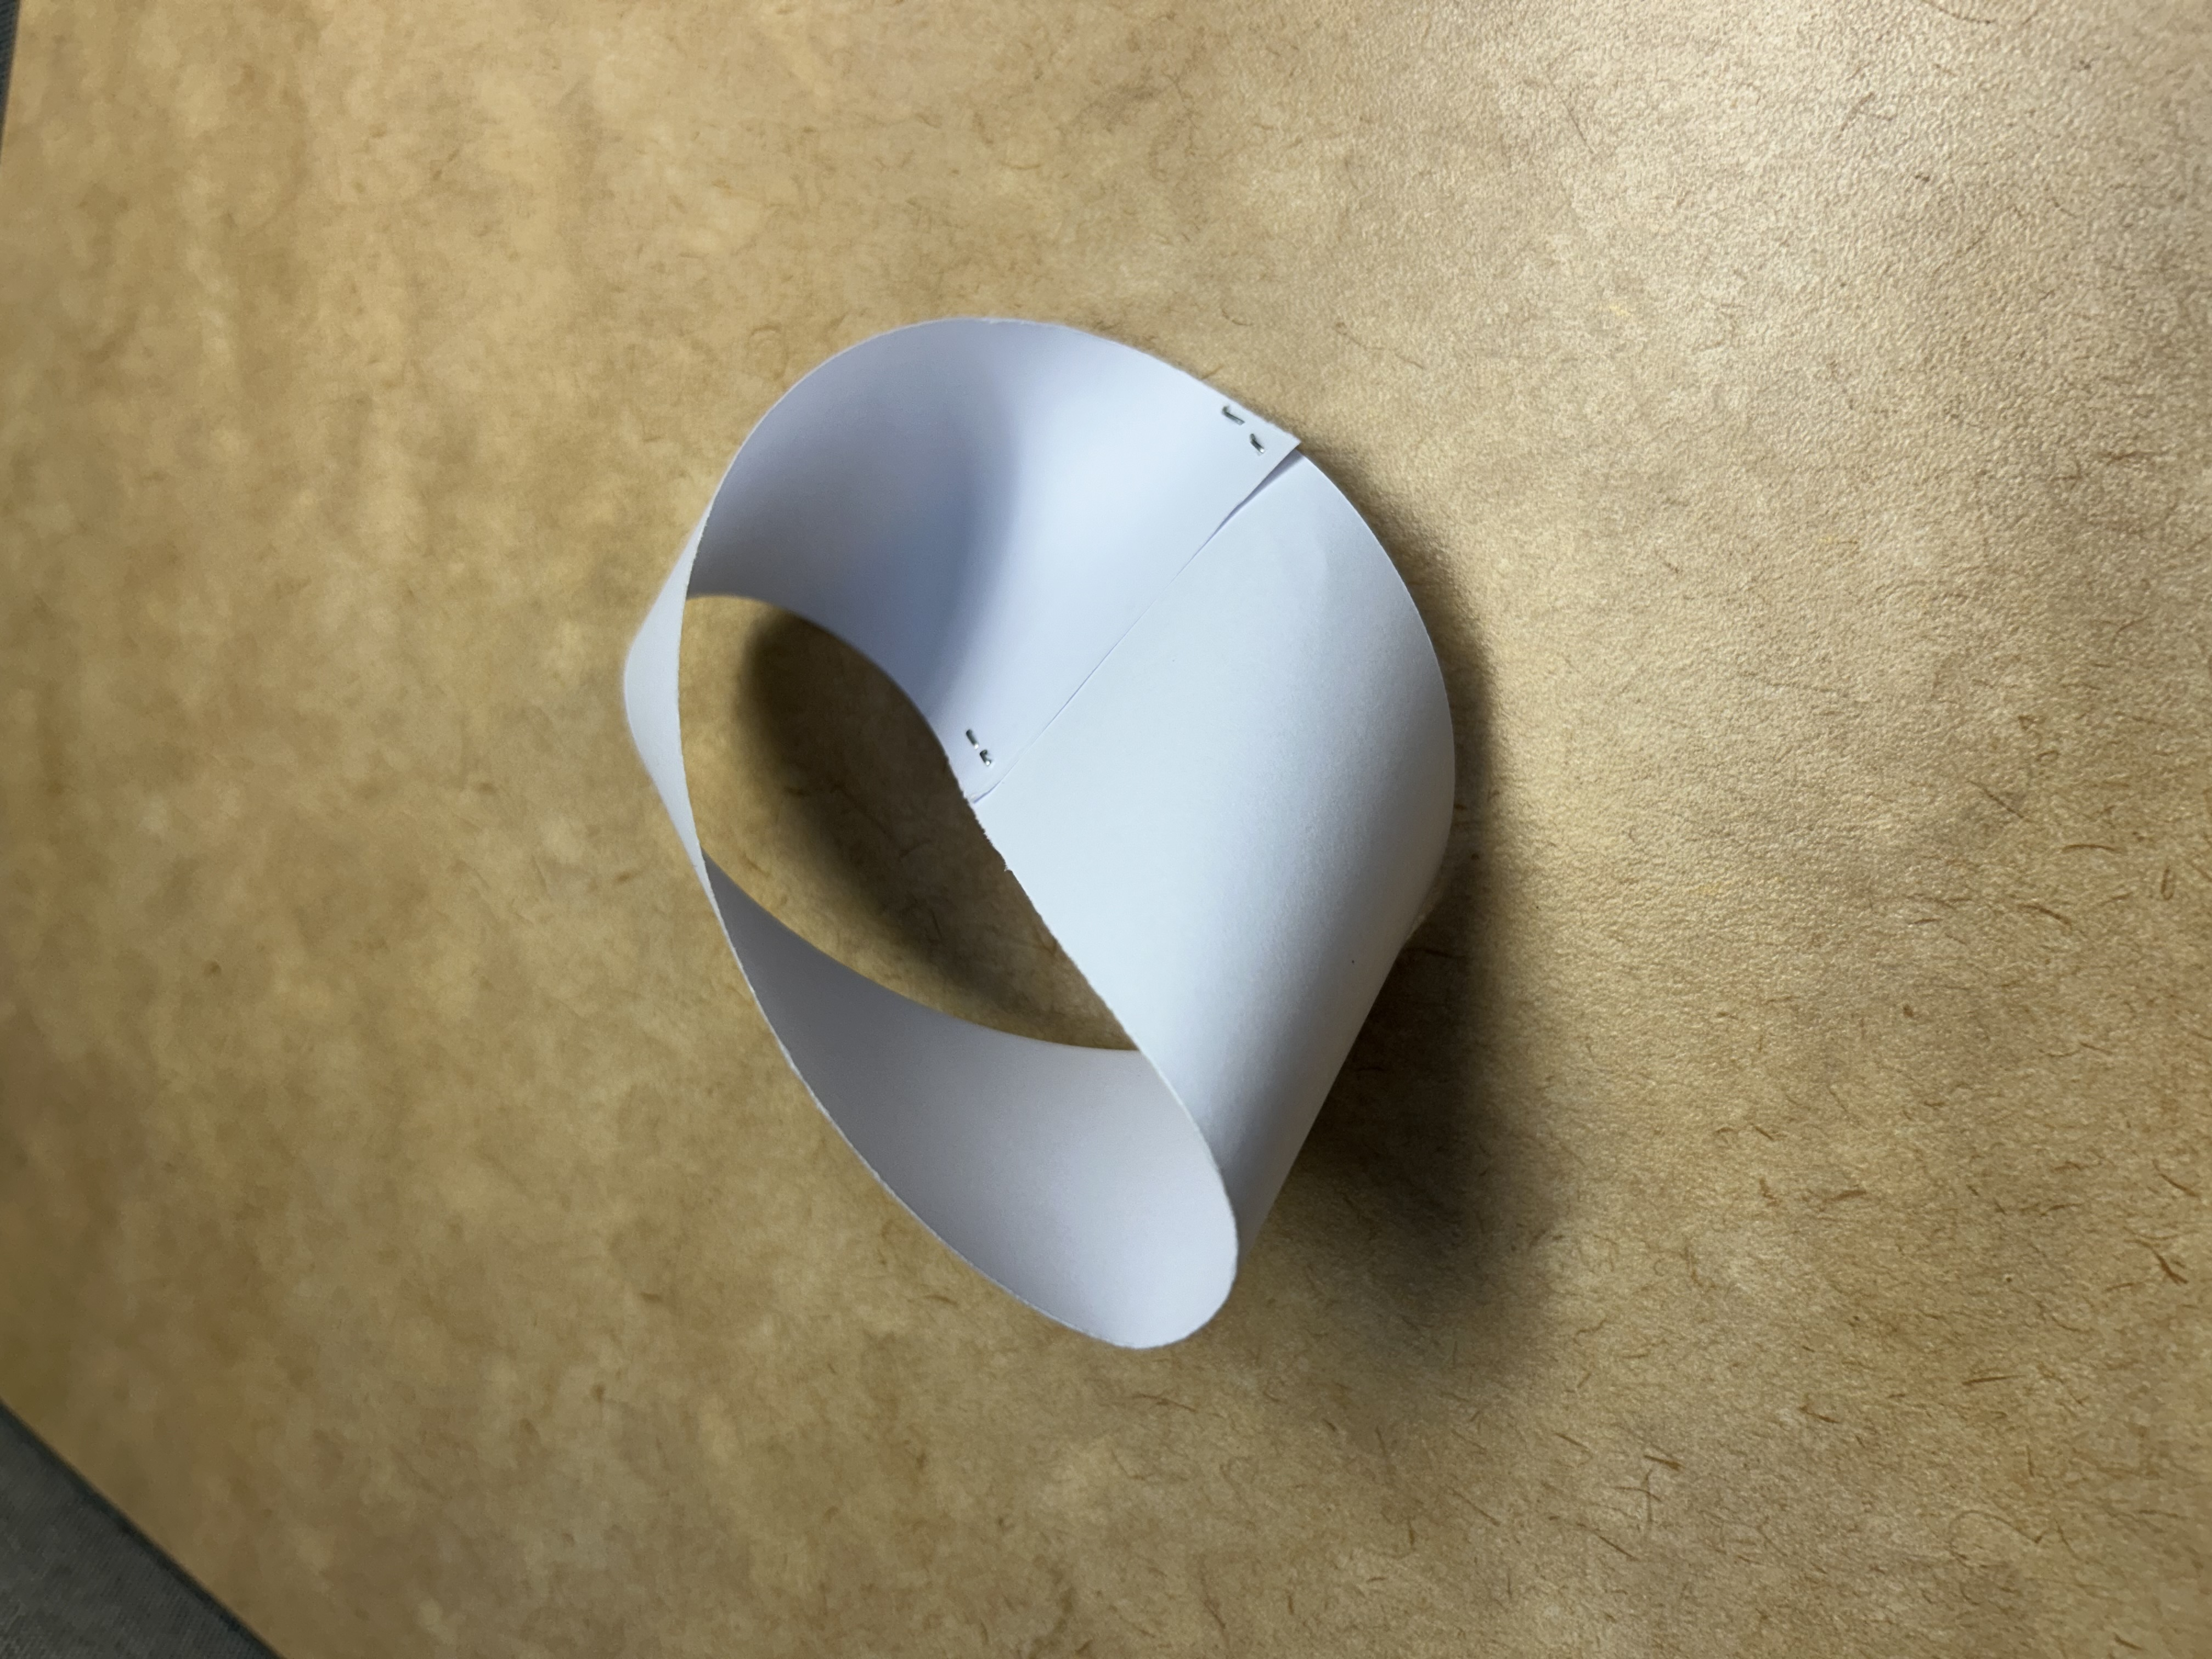
\includegraphics[width=\textwidth]{1twist.jpg}
            \caption{1-strip without a cut}
            \label{fig:fig1}
        \end{subfigure}
        \hfill
        \begin{subfigure}[b]{0.45\textwidth}
            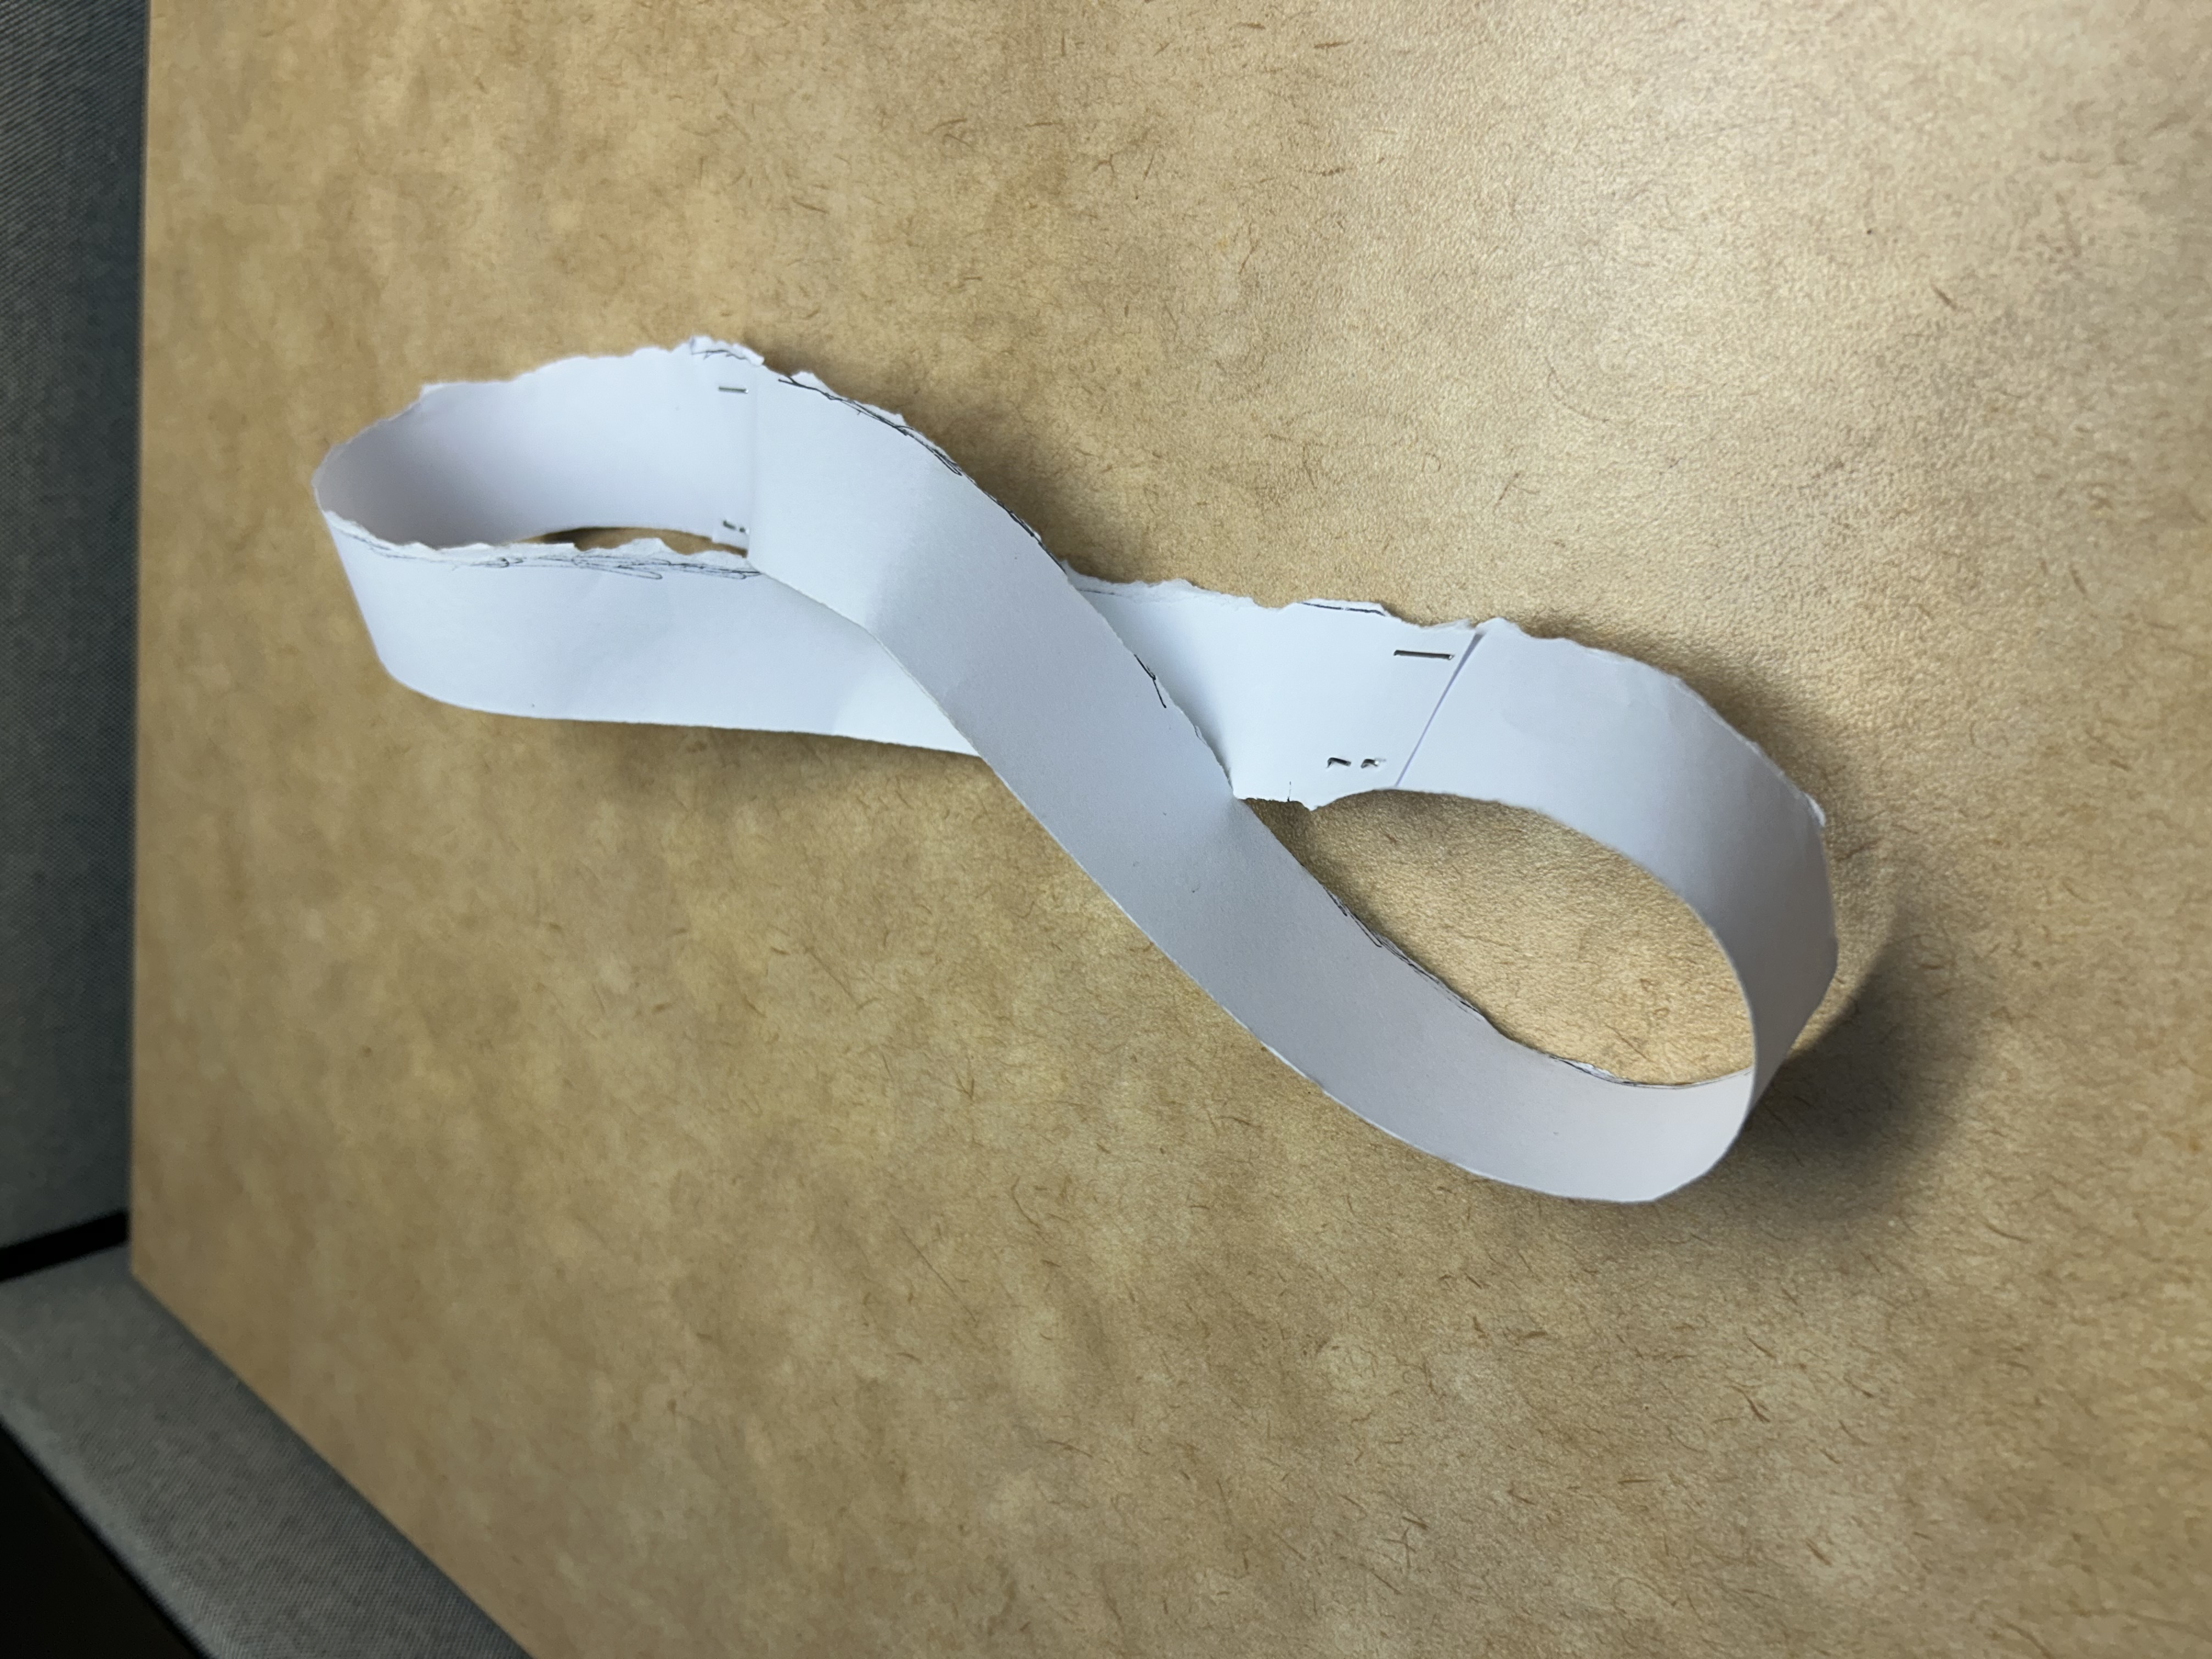
\includegraphics[width=\textwidth]{halfcut.jpg}
            \caption{1/2-cut}
            \label{fig:fig2}
        \end{subfigure}
        \begin{subfigure}[b]{0.45\textwidth}
            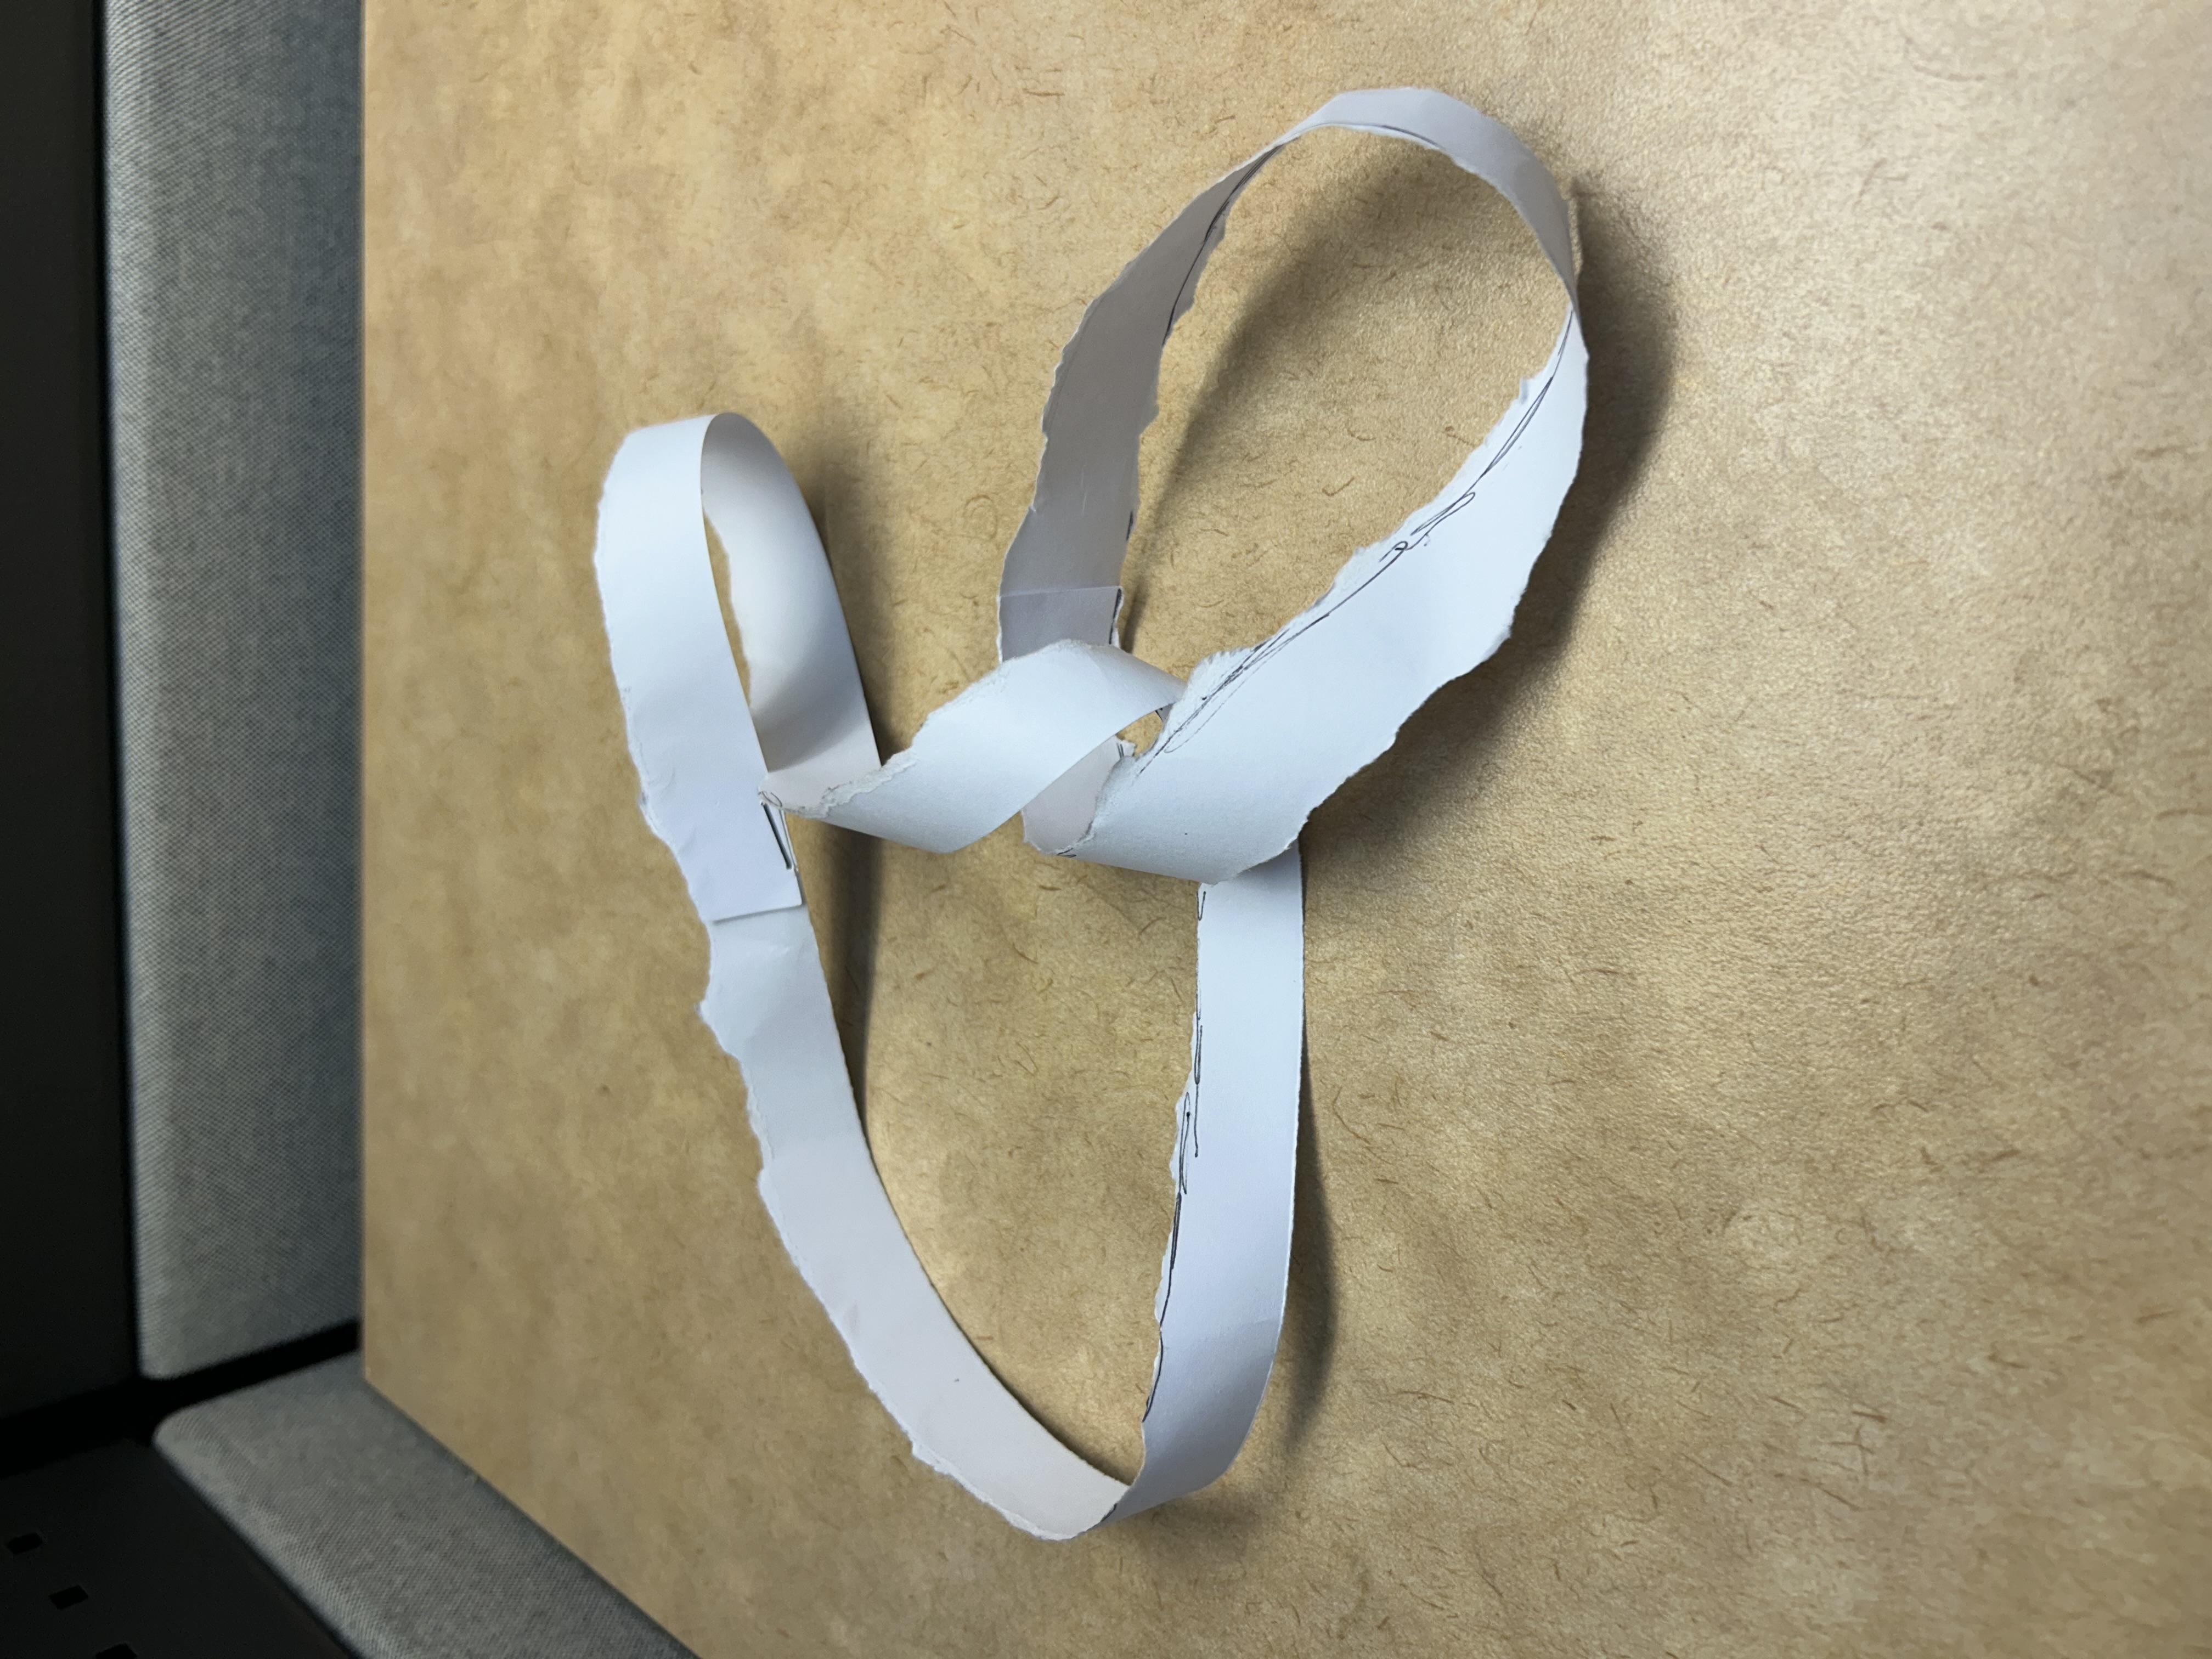
\includegraphics[width=\textwidth]{thirdcut.jpg}
            \caption{1/3-cut}
            \label{fig:fig3}
        \end{subfigure}
    \end{figure}

    In conclusion, the 1/2-cut yields a single 4-twist band and 
    the 1/3-cut yields a 1-twist band and a 4-twist band. 
    
    The discrepency between my conjecture and the experimental result 
    seems to come from the fact that the direction of the 'flip' 
    changes the topological property of the strip. 
\end{proof}

\end{document}